\newpage
\section{Simulation Analysis}
\label{sec:simulation}


\subsection{Exercise 1}
\label{Exercise 1}

%---------------Simulation Analysis Exercise 1--------------------------------------------------------%
In this section we proceed to do the anlysis of the circuit through the use of the Ngspice simulation programm. In figure~\ref{fig:circuit_simulation} we have the circuit that was inputed into Ngspice (and also the considered current flows and nodes). The file can be found at the $sim$ folder inside the $T2$ folder.

\begin{figure}[!ht] \centering
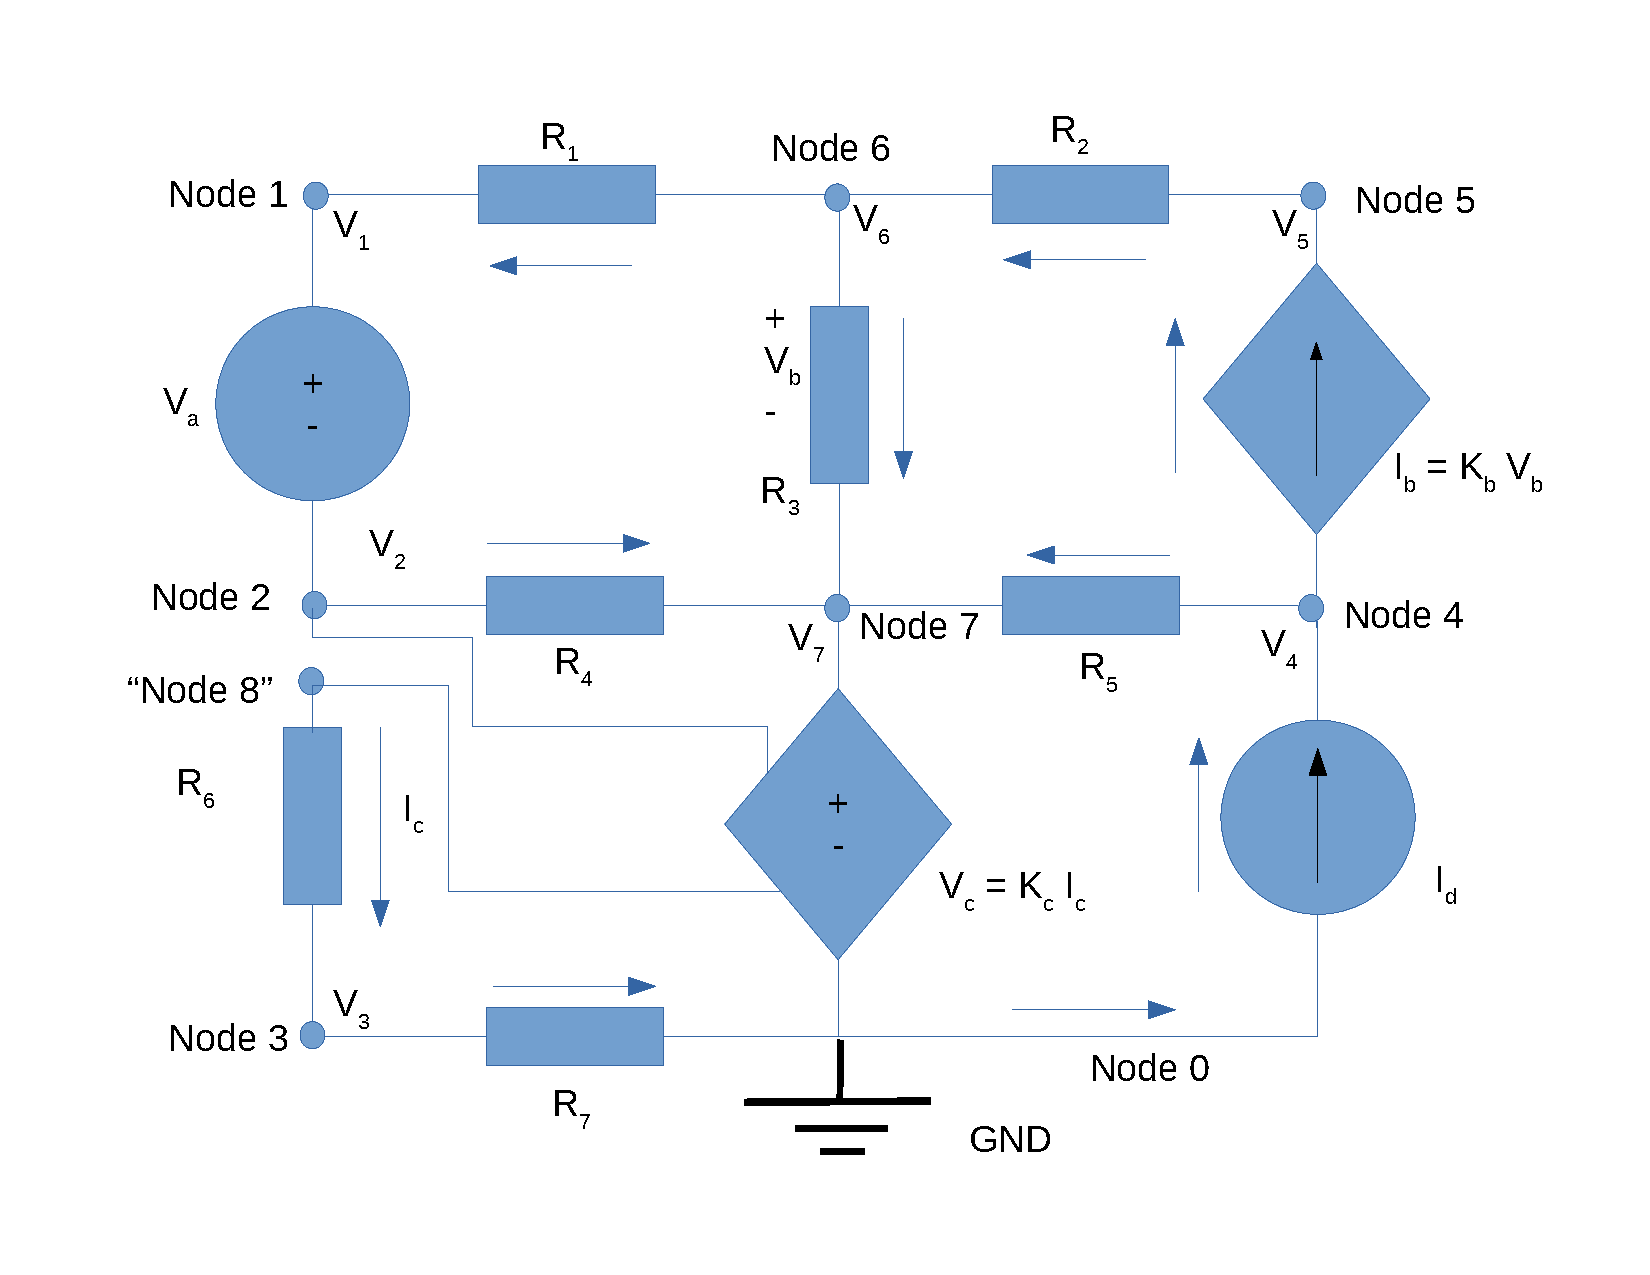
\includegraphics[width=0.8\linewidth]{circuit_simulation.pdf}
\caption{Considered circuit for Ngspice simulation}
\label{fig:circuit_simulation}
\end{figure}

$V_9$ refers to an extra ficticious node created specifically for the Ngspice simulation, and it is below $0(GND)$ and above resistor R6 as it can be seen above in figure~\ref{fig:circuit_simulation}.The reason this node is necessary is because when creating a current controlled voltage source, Ngspice gets the current value by refering to a voltage source from where the current goes through. Since $I_d$ does not go through any voltage source in the circuit (does not go through $V_s$) we used this extra node to create a voltage source of 0$V$ (Which can be confirmed since $V_9 = $GND$ = 0$) from which we are certain $I_d$ is passing by. 

Table~\ref{tab:op} shows the simulated operating point results for the circuit
under analysis given the values found on Table~\ref{tab:op}. The variables representation and format are automatically determined by Ngspice.

\begin{table}[!ht]
  \centering
  \begin{tabular}{|l|r|}
    \hline    
    {\bf Name} & {\bf Value [A or V]} \\ \hline
    @c1[i] & 0.000000e+00\\ \hline
@gib[i] & -2.45467e-04\\ \hline
@r1[i] & 2.344922e-04\\ \hline
@r2[i] & 2.454667e-04\\ \hline
@r3[i] & 1.097445e-05\\ \hline
@r4[i] & 1.220071e-03\\ \hline
@r5[i] & 2.454667e-04\\ \hline
@r6[i] & 9.855785e-04\\ \hline
@r7[i] & 9.855785e-04\\ \hline
v1 & 5.242048e+00\\ \hline
v2 & 5.002985e+00\\ \hline
v3 & 4.499645e+00\\ \hline
v5 & 5.036927e+00\\ \hline
v6 & 5.789615e+00\\ \hline
v7 & -1.98352e+00\\ \hline
v8 & -2.97405e+00\\ \hline
v9 & 0.000000e+00\\ \hline

  \end{tabular}
  \caption{Operating point. A variable preceded by @ is of type {\em current}
    and expressed in Ampere; other variables are of type {\it voltage} and expressed in
    Volt. (the g in "gib" refers to the Ngspice notation of a voltage controlled current source)}
  \label{tab:op}
\end{table}

We can get all the missing values given the equations showed in section~\ref{sec:analysis}.

\begin{equation}
  V_c = V_7
  \label{eq:1}
\end{equation}

\begin{equation}
  V_b = V_6 - V_7
  => V_b = -3.3943*10^{-2} V
\end{equation}

From Table~\ref{tab:op} we can directly get the value of $I_d$:

\begin{equation}
  I_d = @r6[i]
\end{equation}

With this we have finalized the circuit anlysis through simulation with Ngspice.












